\subsection{Cấu trúc dữ liệu biểu diễn đồ thị}
\subsubsection{Thiết kế phần mềm}
\textit{Đồ thị các thành phần phụ thuộc (Module Dependency Graphs)} \\
Một trong những nhiệm vụ quan trọng trong thiết kế phần mềm đó là chia chương trình
thành nhiều thành phần hoặc module khác nhau để tiện cho việc phát triển mà mở rộng
cũng như bảo trì sau này. Việc hiểu được sự tương tác giữa các modules trong một 
chương trình tương tác với nhau như thế nào là cực kì quan trọng không chỉ trong việc 
thiết kế chương trình mà còn trong việc kiểm thử và bảo trì nữa. Một đồ thị các thành 
phần phụ thuộc giúp ích rất nhiều trong việc này. Trong đồ thị các thành phần phụ thuộc 
(dependencies), mỗi đỉnh biểu thị một module, một cạnh nối có hướng chỉ sự phụ thuộc 
của module này vào module kia. Một ví dụ về đồ thị biểu diễn sự phụ thuộc của các modules
trong một ứng dụng web: 
\begin{figure}[H] % places figure environment here   
    \centering % Centers Graphic
    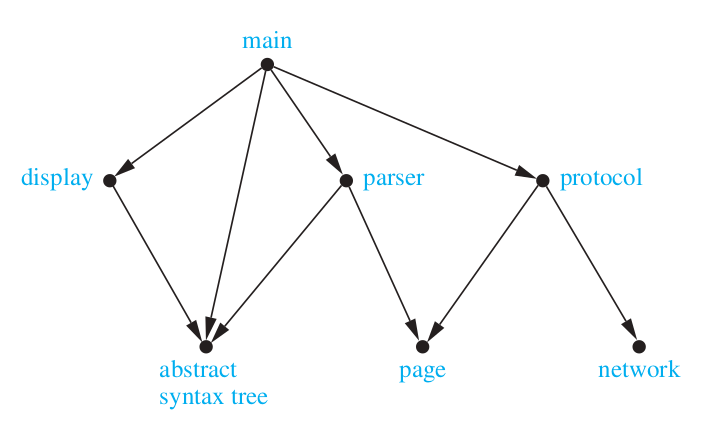
\includegraphics[width=0.6\textwidth]{assets/web_grp.png} 
    \caption{Ví dụ đồ thị sự phụ thuộc của các modules
    trong một ứng dụng web} % Creates caption underneath graph
    \label{fig:gr_1.2.1}
\end{figure}

\subsubsection{Mạng giao thông}
Mô hình đồ thị được sử dụng trong nhiều loại mạng giao thông khác nhau như đường bộ, 
hàng không, mạng đường sắt và mạng chuyển phát. \\

\textit{Định tuyến trong hàng không} \\
Mô hình mạng hàng không có thể được biểu diễn bằng đồ thị với mỗi sân bay là một đỉnh.
Các chuyến bay từ sân bay này tới sân bay khác có thể được biểu diễn bằng một cạnh 
có hướng từ sân bay cất cánh (đỉnh bắt đầu) đến sân bay hạ cánh (đỉnh kết thúc). \\

\textit{Mạng đường bộ} \\
Mô hình đồ thị có thế được sử dụng để biểu diễn mạng đường bộ mà trong đó các đỉnh 
thể hiện các giao lộ và các cạnh thể hiện đường đi. Khi tất cả các cong đường trong mạng 
đều là đường 2 chiều thì ta có thể biểu diễn mạng bằng một đơn đồ thị vô hướng. Tuy 
nhiên trong thực tế ta thường gặp trong mạng giao thông thì một số đường là 2 chiều
và một số khác là 1 chiều. Để biểu diễn mạng này ta dùng cạnh vô hướng để biểu diễn 
đường 2 chiều và cạnh có hướng để biểu diễn đường một chiều.

\subsubsection{Mạng sinh học}
Nhiều khía cạnh của khoa học sinh học có thể được mô hình hóa bằng cách sử dụng đồ thị.\\
\textit{Đồ thị chồng chéo ngách trong hệ sinh thái} \\
Đồ thị được sử dụng trong nhiều mô hình liên quan đến sự tương tác của các loài động vật khác nhau. \\
Ví dụ, sự cạnh tranh giữa các loài trong hệ sinh thái có thể được mô hình hóa bằng cách sử dụng đồ thị chồng chéo thích hợp. Mỗi loài được biểu diễn bằng một đỉnh. Một cạnh vô hướng nối hai đỉnh nếu hai loài đại diện bởi các đỉnh này cạnh tranh (nghĩa là một số nguồn thức ăn mà chúng sử dụng là giống nhau). 
Đồ thị chồng chéo ngách là một đồ thị đơn giản vì không cần vòng lặp hoặc nhiều cạnh trong mô hình này. Biểu đồ trong Hình 11 mô hình hệ sinh thái của một khu rừng. Từ biểu đồ này, chúng ta thấy rằng sóc và gấu trúc cạnh tranh nhưng quạ và chuột thì không.
\begin{figure}[H] % places figure environment here   
    \centering % Centers Graphic
    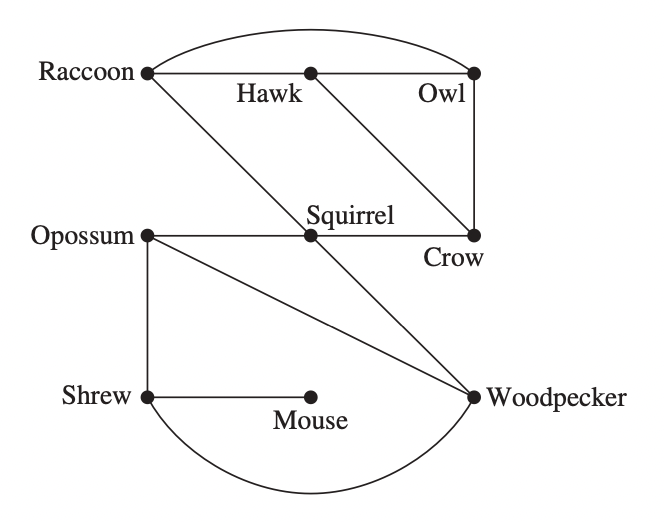
\includegraphics[width=0.5\textwidth]{assets/dothi_chongcheongach.png} 
    \caption{Đồ thị chồng chéo ngách} % Creates caption underneath graph
\end{figure}

\textit{Đồ thị tương tác protein} \\
Tương tác protein trong tế bào sống xảy ra khi hai hoặc nhiều protein trong tế bào đó liên kết với nhau để thực hiện một chức năng sinh học. Bởi vì các tương tác protein là quan trọng đối với hầu hết các chức năng sinh học, nhiều nhà khoa học đang nghiên cứu để phát hiện ra các protein mới và các tương tác cơ bản giữa các protein. Tương tác protein trong tế bào có thể được mô hình hóa bằng cách sử dụng đồ thị tương tác protein,
một đồ thị vô hướng trong đó mỗi protein được biểu diễn bằng một đỉnh, với một cạnh nối các đỉnh biểu thị từng cặp protein tương tác với nhau. Việc xác định tương tác protein thực sự trong tế bào là một vấn đề khó khăn, vì các thí nghiệm thường tạo ra kết quả dương tính giả, kết luận rằng hai protein tương tác khi chúng thực sự không tương tác. Đồ thị tương tác protein có thể được sử dụng để suy ra thông tin sinh học quan trọng, chẳng hạn như bằng cách xác định các protein quan trọng nhất cho các chức năng khác nhau và chức năng của các protein mới được phát hiện.
\begin{figure}[H] % places figure environment here   
    \centering % Centers Graphic
    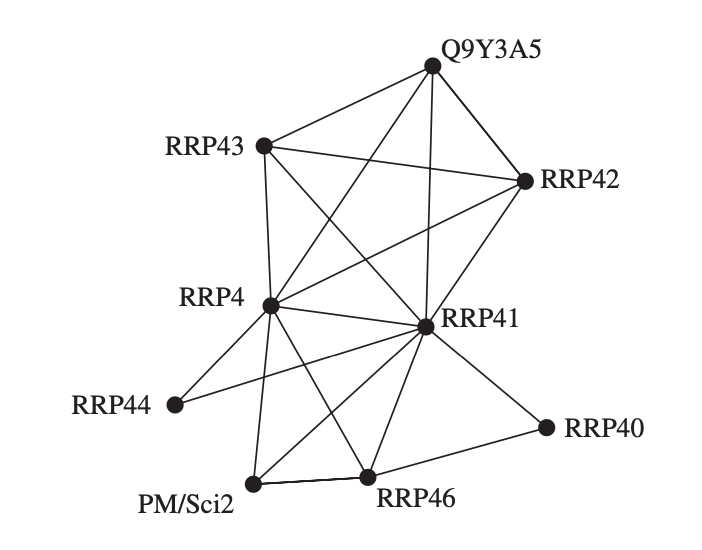
\includegraphics[width=0.5\textwidth]{assets/dothi_tuongtacprotein.png} 
    \caption{Đồ thị tương tác protein} % Creates caption underneath graph
\end{figure}
Bởi vì có hàng ngàn loại protein khác nhau trong một tế bào điển hình, nên đồ thị tương tác protein của một tế bào là cực kỳ lớn và phức tạp. Ví dụ, tế bào nấm men có hơn 6.000 protein, và hơn 80.000 tương tác giữa chúng đã được biết đến, và tế bào người có hơn 100.000 protein, có lẽ khoảng 1.000.000 tương tác giữa chúng. Các đỉnh và cạnh bổ sung được thêm vào đồ thị tương tác protein khi các protein mới và tương tác giữa các protein được phát hiện. Do sự phức tạp của đồ thị tương tác protein, chúng thường được chia thành các đồ thị nhỏ hơn được gọi là mô-đun đại diện cho các nhóm protein có liên quan đến một chức năng cụ thể của tế bào. Hình trên minh họa một mô-đun của đồ thị tương tác protein được mô tả trong [Bo04], bao gồm phức hợp của các protein phân loại RNA trong tế bào người. Để tìm hiểu thêm về đồ thị tương tác protein, hãy xem [Bo04], [Ne10] và [Hu07].

\subsubsection{Mạng ngữ nghĩa}
Các mô hình đồ thị được sử dụng rộng rãi trong việc hiểu ngôn ngữ tự nhiên và trong việc truy xuất thông tin. Hiểu ngôn ngữ tự nhiên (NLU) là chủ đề của máy móc điều khiển để tháo rời và phân tích cú pháp lời nói của con người. Mục tiêu của nó là cho phép máy móc hiểu và giao tiếp như con người. Truy xuất thông tin (IR) là chủ đề thu thập thông tin từ tập hợp các nguồn dựa trên nhiều loại tìm kiếm khác nhau. Sự hiểu biết ngôn ngữ tự nhiên là công nghệ cho phép khi chúng tôi trò chuyện với các nhân viên dịch vụ khách hàng tự động. Những tiến bộ trong NLU được thể hiện rõ khi giao tiếp giữa con người và máy móc liên tục được cải thiện. Khi chúng tôi thực hiện tìm kiếm trên web, chúng tôi tận dụng lợi thế của nhiều tiến bộ trong việc truy xuất thông tin được thực hiện trong những thập kỷ gần đây.\\
Trong các mô hình đồ thị cho các ứng dụng NLU và IR, các đỉnh thường đại diện cho các từ, cụm từ hoặc câu, và các cạnh thể hiện các kết nối liên quan đến ý nghĩa của các đối tượng này.\\
Trong mạng ngữ nghĩa, các đỉnh được sử dụng để biểu diễn các từ và các cạnh vô hướng được sử dụng để kết nối các đỉnh khi một quan hệ ngữ nghĩa giữ giữa các từ này. Quan hệ ngữ nghĩa là quan hệ giữa hai hoặc nhiều từ dựa trên nghĩa của từ. Ví dụ, chúng ta có thể xây dựng một đồ thị trong đó các đỉnh đại diện cho danh từ và hai đỉnh được nối với nhau khi chúng có ý nghĩa tương tự. Ví dụ, tên của các quốc gia khác nhau có ý nghĩa tương tự, tên của các loại rau khác nhau cũng vậy. Để xác định danh từ nào có nghĩa tương tự, có thể kiểm tra phần lớn văn bản. Các danh từ trong văn bản được phân tách bằng dấu liên kết (chẳng hạn như “hoặc” hoặc “và”) hoặc dấu phẩy, hoặc xuất hiện trong danh sách, được cho là có nghĩa tương tự.\\
Ví dụ, xem xét các sách về nông nghiệp, chúng ta có thể xác định rằng các danh từ đại diện cho tên của các loại trái cây như bơ, bưởi, ổi, xoài, đu đủ và mãng cầu xiêm cũng có nghĩa tương tự. Các nhà nghiên cứu thực hiện phương pháp này bằng cách sử dụng British National Corpus, một tập hợp các văn bản tiếng Anh với 100.000.000 từ, tạo ra một biểu đồ với gần 100.000 đỉnh, đại diện cho danh từ và 500.000 liên kết, kết nối các đỉnh đại diện cho các cặp từ có nghĩa tương tự\\
\begin{figure}[H] % places figure environment here   
    \centering % Centers Graphic
    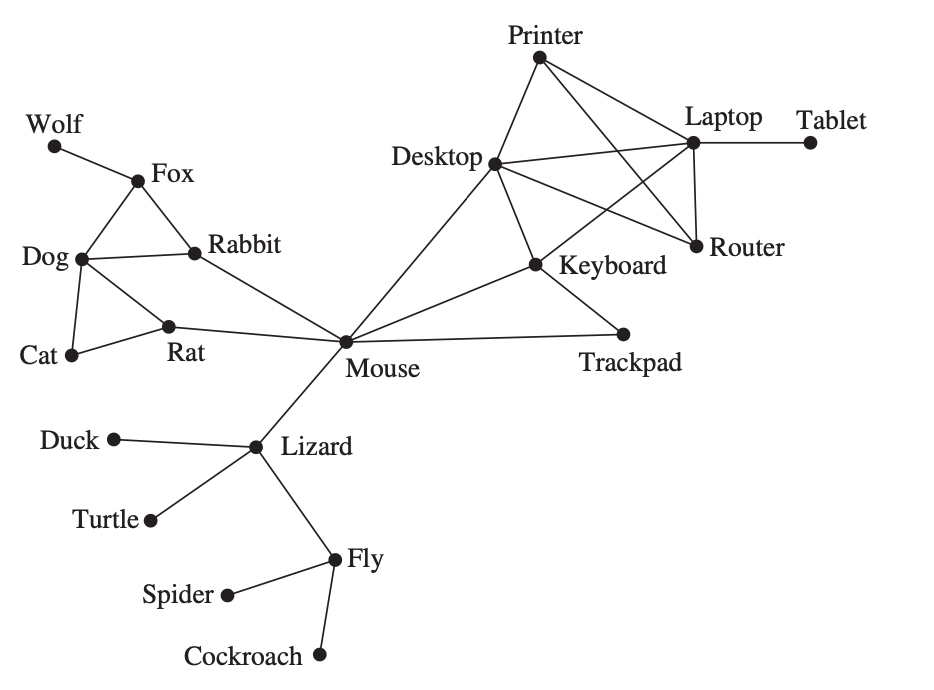
\includegraphics[width=0.8\textwidth]{assets/dothi_mangngunghia.png} 
    \caption{Đồ thị mạng ngữ nghĩa} % Creates caption underneath graph
\end{figure}
Hình trên hiển thị một đồ thị nhỏ trong đó các đỉnh đại diện cho danh từ và các cạnh nối các từ có nghĩa tương tự. Biểu đồ này tập trung xung quanh từ chuột. Biểu đồ minh họa rằng có hai ý nghĩa riêng biệt đối với chuột. Nó có thể đề cập đến một con vật hoặc nó có thể đề cập đến phần cứng máy tính. Khi một chương trình NLU gặp từ mouse trong một câu, nó có thể xem những từ nào có nghĩa tương tự sẽ phù hợp với câu để giúp xác định xem con chuột ám chỉ động vật hay phần cứng máy tính trong câu đó.\\

\subsubsection{Mạng thi đấu}
\textit{Thi đấu vòng tròn} \\
Một giải đấu mà mỗi đội đấu với các đội khác đúng một lần và không cho phép hòa được gọi là giải đấu vòng tròn một lượt. Các giải đấu như vậy có thể được mô hình hóa bằng cách sử dụng đồ thị có hướng trong đó mỗi đội được biểu diễn bằng một đỉnh. Lưu ý rằng (a, b) là một cạnh nếu đội a thắng đội b. Biểu đồ này là một biểu đồ có hướng đơn giản, không chứa vòng lặp hoặc nhiều cạnh có hướng (vì không có hai đội chơi với nhau nhiều hơn một lần). Mô hình đồ thị có hướng như vậy được trình bày trong hình. Chúng tôi thấy rằng Đội 1 là đội bất bại trong giải đấu này,
và Đội 3 bất phân thắng bại.\\
\begin{figure}[H] % places figure environment here   
    \centering % Centers Graphic
    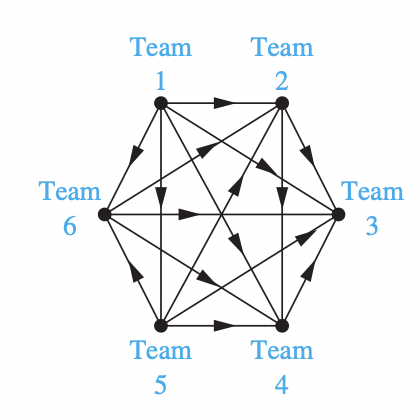
\includegraphics[width=0.6\textwidth]{assets/dothi_thidauvongtron.png} 
    \caption{Thi đấu vòng tròn} % Creates caption underneath graph
\end{figure}
\textit{Thi đấu loại trực tiếp} \\
Một giải đấu mà mỗi thí sinh bị loại sau một lần thua được gọi là giải đấu loại trực tiếp. Các giải đấu loại trực tiếp thường được sử dụng trong thể thao, bao gồm giải vô địch quần vợt và giải vô địch bóng rổ NCAA hàng năm. Chúng ta có thể lập mô hình một giải đấu như vậy bằng cách sử dụng một đỉnh để đại diện cho mỗi trò chơi và một cạnh có hướng để kết nối trò chơi với trò chơi tiếp theo mà người chiến thắng trong trò chơi này đã chơi. Biểu đồ trong hình dưới thể hiện các trò chơi của 16 đội cuối cùng trong năm 2010 NCAA của
giải đấu bóng rổ.
\begin{figure}[H] % places figure environment here   
    \centering % Centers Graphic
    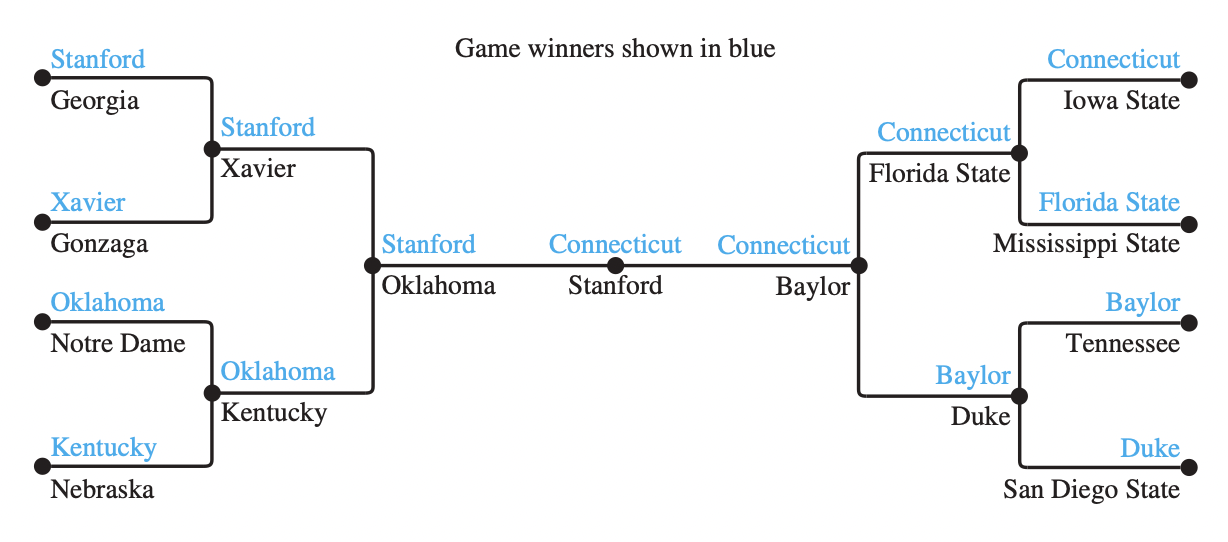
\includegraphics[width=0.7\textwidth]{assets/dothi_thidauloaitructiep.png} 
    \caption{Thi đấu loại trực tiếp} % Creates caption underneath graph
\end{figure}